\documentclass[12pt,openright,a4paper,brazil]{abntex2}

\usepackage{ders-ifro}

\sistema{Nome do sistema}
\versao{1.0.0}
\autor{Nome do autor 1 $<$autor.um@ifro.edu.br$>$ \\ Nome autor 2 $<$autor.dois@ifro.edu.br$>$}
\data{Junho 2016}

\begin{document} 

\imprimircapa

\begin{resumo}
	Este documento apresenta orientações para a elaboração de projetos de sistemas a serem desenvolvidos pelo Instituto Federal de Rondônia -- IFRO. Toda formatação deverá seguir estritamente às normas vigentes da ABNT para projetos de pesquisa quanto às fontes, margens, espaçamentos, elementos pré-textuais, textuais e pós-textuais. 
	
	Para usuários \LaTeX, utilizamos a classe \abnTeX que contém todas as funções necessárias para a construção do documento. A documentação completa é encontrada em \url{https://github.com/abntex/abntex2/wiki/Download} e pode ser utilizada como apoio na elaboração do documento. Entretanto, para estar em conformidade com padrões únicos do IFRO, baixe o arquivo de customização em \url{https://github.com/ifroariquemes/derstex} para adequar os padrões de capa e estruturas. 
	
	\vspace{\onelineskip}
	\noindent
	\textbf{Palavras-chave}: template. dersex. ifro.
	
	\vspace{\onelineskip}
	\centering \color{red} \textbf{** Esta página de resumo não é necessária no documento **}
	
\end{resumo}

\pdfbookmark[0]{\listfigurename}{lof}
\listoffigures*
\cleardoublepage

\pdfbookmark[0]{\listtablename}{lot}
\listoftables*
\cleardoublepage

\begin{siglas}
	\item[ABNT] Associação Brasileira de Normas Técnicas
	\item[abnTeX] ABsurdas Normas para \LaTeX
	\item[dersTeX] Documento de Especificação de Requisitos de Software para \LaTeX
\end{siglas}

\pdfbookmark[0]{\contentsname}{toc}
\tableofcontents*
\cleardoublepage

% ----------------------------------------------------------
% ELEMENTOS TEXTUAIS
% ----------------------------------------------------------
\textual

\chapter*[Introdução]{Introdução}
\addcontentsline{toc}{chapter}{Introdução}

A introdução serve de ponto inicial para o leitor compreender de forma rápida o problema abordado e as motivações que levaram à criação do sistema proposto. Deve ficar muito claro o método atual utilizado no processo sendo tratado (se a forma atual é manual, se há um outro sistema) e enfatizar os pontos mais críticos em que os usuários ou executantes do processo atual sentem mais dificuldades. 

O projetista deve atentar para a definição de um escopo contendo resumidamente as funções do novo sistema e quais dos problemas atuais o software \textbf{NÃO} vai resolver, isto é, que ficarão pendentes para trabalhos futuros, versões futuras ou mesmo aqueles que por algum motivo não possuem desenvolvimento viável (neste caso explicar os critérios que elegeram a inviabilidade). 

Os últimos parágrafos devem resumir a estrutura que se seguirá no documento adiantando ao leitor que assuntos serão abordados em cada capítulo.

Portanto, recomendamos que a introdução contemple os seguintes itens:
\begin{itemize}
	\item problemática;
	\item motivações;
	\item método atual;
	\item pontos críticos;
	\item escopo do sistema proposto;
	\item e estrutura do restante do documento.
\end{itemize}

\chapter{Descrição Geral}

No início deste capítulo, demonstre os resultados esperados com a utilização do sistema proposto. Insista na solução dos problemas críticos enfrentados pelos usuários e outros fatores que visem a valorização do produto.

\textbf{NÃO} utilize esse espaço para:
\begin{itemize}
	\item características tecnológicas como plataforma, arquitetura, e softwares de terceiros;
	\item escopo restritivo (dizer o que o software não fará);
	\item e assuntos relacionados a qualquer seção deste capítulo.
\end{itemize} 

\section{Características dos Usuários}

Defina quem são os usuários em potencial do sistema. Nomeie genericamente pela atribuição e papel de cada um na organização e descreva a atuação deles no processo atual e em que momento o novo sistema entrará em cena. Demonstre como a utilização e integração de todos os envolvidos é pertinente para o bom funcionamento do sistema, e a posição de cada um no programa.

\section{Restrições tecnológicas}

Nesta seção você deve impor as tecnologias necessárias para a construção e implantação do sistema tais como plataformas, dispositivos e requisitos mínimos de hardware. Além disto serão expostos requerimentos de software envolvidos, como máquinas virtuais, bancos dados e softwares de terceiros. Caso uma implementação específica não seja necessária mas sim um atributo tecnológico, como, por exemplo, design responsivo ou banco de dados orientado a objeto, declarar a necessidade desta deixando aberto ao desenvolvedor a escolha da melhor forma de entregar esses requisitos.

\section{Restrições funcionais}

Aqui serão desenroladas as funções que não serão implementadas pelo software apesar de necessárias para a solução do problema em questão. Os motivos para a inviabilidade devem ser demonstrados com clareza.

\section{Pressupostos e Dependências}

Caso seja necessário, esta seção deve ser utilizada para dissertar sobre hipóteses em qualquer nível, operacional ou pessoal, que possa atrapalhar o bom andamento do desenvolvimento do produto, como a aprovação de um superior, participação de usuários durante testes e qualquer outro cenário que possa vir a se tornar um risco para o funcionamento do sistema e à execução do projeto.

\chapter{Requisitos Específicos}

Através das observações realizadas quanto às demandas solicitadas, levando em consideração aquilo que o departamento demandante necessita e quanto as informações gerenciadas afetam na organização, seguirá aqui a escrita de um capítulo para descrição dos requisitos necessários para satisfazer os pedidos realizados. Para cada requisito funcional elegido, haverá obrigatoriamente ao menos um requisito não-funcional e opcionalmente requisitos de interface. 

Um \emph{requisito funcional} representa uma função generalizada que o software terá de desempenhar; \emph{requisitos não-funcionais} definem as regras que regerão determinadas funções do sistema como validações, questões de segurança, atributos para persistência e regras de negócio; enquanto que cada \emph{requisito de interface} indica uma necessidade identificada pelo projetista como sendo essencial para a composição da interação humano-computador -- IHC (principalmente nos casos em que se deseja causar menor impacto visual ao criar formulários com design semelhante àquele que os usuário já estão familiarizados).

Cada requisito funcional será identificado nos documentos pelas letras RF seguidas de um numeral sequencial e único: RF1, RF2, ..., RFn.

Os requisitos não-funcionais e de interface serão identificados pelas siglas RNF e RI respectivamente, seguidas pelo índice do RF ao qual se referencia e depois por numeral sequencial e único: RNF1.1, RNF1.2, ..., RNF1.n; RI1.1, RI1.2, ..., RI1.n. 

O nome dos RF devem iniciar por verbos no infinitivo (terminados em ar, er, ir) e possuir contexto único entre todos os RF do sistema:

\begin{itemize}
	\item RF1 - Cadastro de aulas (inválido, primeira palavra é um substantivo)
	\item RF2 - Cadastrar cliente (válido)
	\item RF3 - Alterar cadastro do cliente (inválido, contexto que trata de ``cadastro do cliente'' já existe)
\end{itemize}

A tabela \ref{tab:rf} mostra um modelo de tabela montada para cada RF elicitado. No decorrer do projeto, caso seja necessário referenciar qualquer item, RF, RNF ou RI, toda a cadeia de caracteres será utilizada como identificação única, sigla e números.

\begin{table}
	\caption{Exemplo de tabela descritiva de requisito funcional}
	\label{tab:rf}
	\centering
	\begin{tabular}{|p{.2\linewidth}|p{.75\linewidth}|}
		\hline
		\multicolumn{2}{|l|}{
			\textbf{RF1 - Nome do requisito funcional}
		} \\
		\multicolumn{2}{|l|}{
			\textbf{Descrição:} Texto descrevendo o contexto do requisito funcional.
		} \\ \hline
		\multicolumn{2}{|c|}{
			\textbf{Requisitos não-funcionais}
		} \\ \hline
		RNF1.1 & Requisito não-funcional 1.1 \\ \hline
		RNF1.2 & Requisito não-funcional 1.2 \\ \hline
		RNF1.3 & Requisito não-funcional 1.3 \\ 
		\hline
		\multicolumn{2}{|c|}{
			\textbf{Requisitos de interface}
		} \\ \hline
		RI1.1 & Requisito de interface 1.1 \\ \hline
		RI1.2 & Requisito de interface 1.2 \\ \hline
		RI1.3 & Requisito de interface 1.3 \\
		\hline
	\end{tabular}
\end{table}


\chapter{Diagramas}

O uso de diagramas é essencial para a compreensão profunda tanto do problema quanto da solução sendo desenvolvida. Em informática é comum recorrer ao Diagrama Entidade-Relacionamento (DER) e/ou à Linguagem de Modelagem Unificada (UML) durante o projeto de sistemas. Para elaboração deste documento de especificação, ambas as técnicas podem ser invocadas, sendo que a utilização de DER torna obrigatória a aplicação de um dicionário de dados, enquanto que ao usar UML requeremos ao menos um diagrama de Caso de Uso e sua descrição formal. 

A seleção de quaisquer outros digramas é opcional e válida na composição deste documento, desde que devidamente descritos e que sejam relevantes ao projeto entregando novas perspectivas que, sem estes, seria mais complexo ou mesmo impossível de se perceber.

\section{Casos de Uso}

O digrama de caso de uso deve contemplar as funções globais do sistema fazendo alusão aos requisitos funcionais levantados no capítulo anterior. Cada RF deve gerar ao menos um caso de uso (UC) os quais devem estar dispostos e disponíveis aos atores exatamente como demandado pelos RNF. Processos fora dos limites do sistema (system boundary) também podem ser modelados se o projetista julgar necessário. Um exemplo pode ser visualizado na figura \ref{fig:uc}.

\begin{figure}
	\centering
	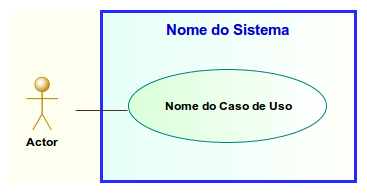
\includegraphics[width=.6\linewidth]{uc}
	\caption{Exemplo de diagrama de caso de uso}
	\label{fig:uc}
\end{figure}


Assim como nos requisitos, UC também possuem um número de identificação sequencial e único utilizado em sua descrição formal e referenciamento no documento, porém não aparecem nos digramas. As regras de nomenclatura seguem as mesmas que de RF. O início da descrição de cada UC deve ser efetuado em uma nova página.

Uma das características abordadas pelos UC é a prioridade de desenvolvimento por função. Mantenha com prioridade mais alta os primeiros módulos a serem programados, como aqueles que são dependência de outros. Veja na tabela \ref{tab:uc-pri} os valores de prioridades.

A frequência de uso de um UC pode variar inclusive inversamente à sua prioridade de desenvolvimento dependendo do escopo do projeto. Tomando como exemplo um site de notícias, o cadastro da notícia feito pelo administrador é menos utilizados que a visualização da notícia feita pelos usuários públicos. Uma vez que o cadastro é realizado uma vez, a visualização é feita milhares de vezes, ou seja, para o sistema a frequência de uso do cadastro é baixa, enquanto que a visualização tem frequência alta. Para atribuição de uma frequência de uso razoável, deve-se pensar num período entre uma semana e um ano de uso normal do sistema e inferir tempos de uso a cada função, então utilize os itens da tabela \ref{tab:uc-freq} para determinar o uso.

\begin{table}[!h]
	\caption{Valores de prioridades de desenvolvimento para casos de uso}
	\label{tab:uc-pri}
	\setlength\extrarowheight{5pt}
	\begin{tabular}{p{.2\linewidth}p{.75\linewidth}}
		\hline
		\textbf{Prioridade} & \textbf{Descrição} \\
		\hline
		1 - Urgente & Função extremamente necessária para o desenvolvimento de partes críticas do sistema, existe dependência de sua existência para que funções críticas possam ser criadas \\
		2 - Crítica & Função que se refere a um dos problemas críticos enfrentados pelos usuários, devem ser estar no topo das funções a implementar e disponibilizadas para produção o mais rápido possível \\
		3 - Importante & Função importante na solução de problemas críticos que deve constar ainda nas versões iniciais do sistema \\
		4 - Relevante & Função relevante para regras de negócio triviais, deve estar no sistema até à versão final \\
		5 - Desejável & Função sem muita importância para o sistema como um todo, sua ausência não afetará na solução dos problemas críticos, porém seu desenvolvimento é desejável para um futuro ainda indeterminado \\
		\hline
	\end{tabular}
\end{table}

\begin{table}[h]
	\caption{Valores de frequência de uso para casos de uso}
	\label{tab:uc-freq}
	\setlength\extrarowheight{5pt}
	\begin{tabular}{p{.2\linewidth}p{.75\linewidth}}
		\hline
		\textbf{Frequência} & \textbf{Descrição} \\
		\hline
		Alta & Utilização maior que 15\% do tempo \\
		Média & Utilização de 5\% a 15\% do tempo \\
		Baixa & Utilização de até 5\% do tempo \\
		\hline
	\end{tabular}
\end{table}

\clearpage
\subsection{UC1 - Nome do Caso de Uso}
\newcounter{uc1}

\begin{longtable}{p{.25\linewidth}p{.7\linewidth}}
\textbf{Objetivo:} & Descreva o objetivo do caso de uso. \\
\textbf{Requisitos:} & Identifique os requisitos aos quais este UC está relacionado (e.g. RF1, RF2). \\
\textbf{Atores:} & Identifique os atores envolvidos no UC. \\
\textbf{Prioridade:} & Identifique qual a prioridade de desenvolvimento deste UC (ver~tabela~\ref{tab:uc-pri}). \\
\textbf{Pré-condições:} & Condições necessárias para que UC seja executado. \\
\textbf{Pós-condições:} & Condições do sistema após a execução do UC. \\
\textbf{Frequência de uso: } & Identifique a frequência de uso deste UC (ver~tabela~\ref{tab:uc-freq}).\\
\textbf{Campos:} & Identifique os campos necessários no contexto sendo trabalho neste UC. \\
\textbf{Fluxo principal:} & 
Defina um passo-a-passo das principais ações que o usuário deve tomar dentro deste UC considerando um caso de sucesso (sempre iniciar pelo ator).
\begin{enumerate}[label=\alph*)]
	\item \label{UC1:FP:a} Ator faz isso;
	\item Sistema responde;
	\item \label{UC1:FP:c} Ator \hyperref[UC1:FA:A1]{(A1)} \hyperref[UC1:FA:A2]{(A2)} faz isso;
	\item Sistema \hyperref[UC1:FE:E1]{(E1)} responde;
	\item O caso de uso é encerrado.
\end{enumerate} \\
\textbf{Fluxo alternativo:} & 
Defina caminhos alternativos que o usuário pode iniciar por vontade própria dentro do UC (sempre iniciar pelo ator).
\vspace{\onelineskip}
\label{UC1:FA:A1} A1 - muda de ideia
\begin{enumerate}[label=\alph*)]
	\item Ator muda de ideia;
	\item Sistema responde;
	\item Retorna ao passo \ref{UC1:FP:c} do fluxo principal.
\end{enumerate} 
\label{UC1:FA:A2} A2 - cancela operação
\begin{enumerate}[label=\alph*)]
	\item Ator cancela operação;
	\item Sistema responde;
	\item O caso de uso é encerrado.
\end{enumerate} \\
\textbf{Fluxo de exceção:} &
Defina cenários em que o sistema pode disparar erros causados pelo usuário ou qualquer ação dentro da UC que tenha sido iniciada por decisão do sistema (sempre iniciar pelo sistema).
\vspace{\onelineskip}
\label{UC1:FE:E1} E1 - captura erro
\begin{enumerate}[label=\alph*)]
	\item Sistema captura erro e mostra mensagem;
	\item Retorna ao passo \ref{UC1:FP:c} do fluxo principal.
\end{enumerate} \\
\textbf{Validações:} & Defina como os campos serão validados e todos os casos que podem fazer disparar fluxos de exceção. \\
\textbf{Protótipos de telas:} & \\
\multicolumn{2}{p{\linewidth}}{
	Insira imagens de protótipos de telas que possam realizar as ações descritas no UC contendo os requisitos de interface dos RF relacionados.
} \\
\end{longtable} 

\clearpage
\section{Classes}

\subsection{Nome da Classe}

\section{Atividades}

\section{Sequências}

\chapter{Resultados esperados}

\chapter{Cronograma}

\chapter{Orçamento}

\chapter{Cronograma}

\chapter{Orçamento}
Discriminar os recursos necessários para o desenvolvimento do projeto.

\phantompart

\chapter*[Considerações finais]{Considerações finais}
\addcontentsline{toc}{chapter}{Considerações finais}

\postextual

\bibliography{../assets/ders-ifro}

\phantompart

\printindex

\end{document}